A well-studied example of complex behavior arising from simple mechanisms is the coexistence of synchrony and asynchrony within a system of identical coupled oscillators, a phenomenon known as a chimera state \cite{Kuramoto2002,Abrams2004}.
The existence of these chimera states is surprising, as they represent asymmetry within symmetric systems.
One of the simplest systems which produces chimera states is the Abrams model which consists of two populations of identical oscillators with a stronger coupling strength within the populations than between them \cite{Abrams2008}.
The system is described by the following:
\begin{equation}
  \label{eq:abrams}
  \dv{\theta_{i}^{\sigma}}{t}
  =
  \omega
  +
  \sum_{\sigma' = 1}^{2} \frac{K_{\sigma \sigma'}}{N_{\sigma'}} \sum_{j = 1}^{N_{\sigma'}} \sin(\theta_{j}^{\sigma'} - \theta_{i}^{\sigma} - \alpha),
\end{equation}
where
\begin{equation*}
  K
  =
  \bmqty{\mu & \nu \\ \nu & \mu}
  \qand
  \sigma \in \Bqty{1, 2}.
\end{equation*}
In this model, $\mu$ represents the intra-population strength, and $\nu$ represents the inter-population strength, with $\mu > \nu$.
Time can be scaled such that $\mu + \nu = 1$.
If $\mu - \nu$ is not too large, and $\alpha$ is not too much less than $\frac{\pi}{2}$, then this system can produce chimera states.
\Cref{fig:abrams} shows a simulation of the Abrams model on two populations of 128 oscillators.
\begin{figure*}[ht]
  \centering
  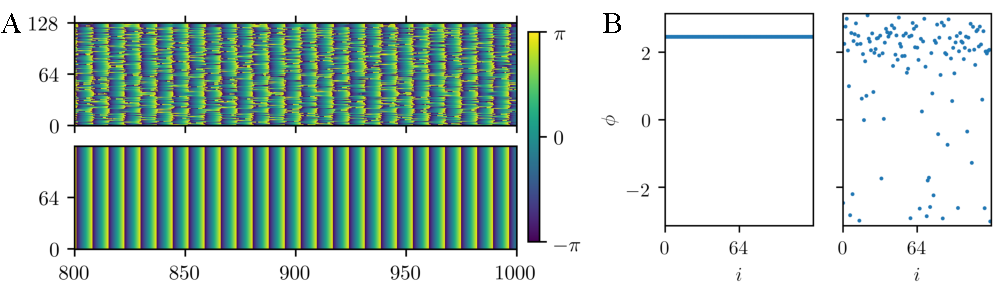
\includegraphics[width=\textwidth]{figure/abrams.pdf}
  \caption[Abrams simulation]{A simulation of the Abrams model for two populations of 128 oscillators.
    We employed a 4th-order Runge-Kutta solver ($\dd{t} = 0.01$, $t_{\text{max}} = 1000$).
    A. Time series of the simulation for $t \in \pqty{800, 1000}$.
    B. Snapshot at $t \approx 800$.
  }
  \label{fig:abrams}
\end{figure*}

An analogous system has recently been analyzed in the physical world \cite{Martens2013}.
Two swinging platforms were coupled together with springs of variable spring constant $\kappa$, and 15 metronomes---all tuned to the same frequency---were placed on each platform.
The metronomes on the same platform are coupled through the motion of the swing, which heavily influences the motion of the metronomes, represented in the Abrams model by $\mu$.
The metronomes on opposite platforms are coupled through the springs, which is a much weaker interaction, represented in the Abrams model by $\nu$.
For a wide range of values of $\kappa$, all of the metronomes on one platform would synchronize, while the metronomes on other platform would remain asynchronous.

While chimera states may present themselves obviously when observed in a plot or the physical world, they can be harder to pin down analytically.
In order to do so, we will investigate a system of $M$ communities of nonlocally-coupled oscillators, and we sample their phases at times $t \in \bqty{1, \ldots, T}$.
A useful pair of measures for detecting the presence of a chimera state are the chimera-like index $\chimera$ and the metastability index $\meta$ \cite{Shanahan2010,Hizanidis2016}.
To develop these two measures, we start with the order parameter $\ordparam_{c}(t) = \abs{\expval{e^{i \phase_{k}(t)}}_{k \in C}}$, where $\phase_{k}$ is the phase of oscillator $k$, and $\ev{f}_{k \in C}$ is the average of $f$ over all $k$ in community $C$.
The order parameter $\ordparam$ indicates the instantaneous synchrony of a community (how similar the phases of the oscillators are to the others in $C$), and not its overall coherence (how similar the trajectories of the oscillators are).
From this, we define the two measures:
\begin{align}
  \label{eq:chimera}
  \chimera
  &=
    7 \times \expval{\sigma_{\text{chi}}}_{T}, \\
  \label{eq:metastability}
  \meta
  &=
    12 \times \expval{\sigma_{\text{met}}}_{C},
\end{align}
where
\begin{equation}
  \sigma_{\text{chi}}(t)
  =
  \frac{1}{M - 1} \sum_{c \in C}\pqty{\ordparam_{c}(t) - \expval{\ordparam_{c}}_{C}}^{2},
\end{equation}
and
\begin{equation}
  \sigma_{\text{met}}(c)
  =
  \frac{1}{T - 1} \sum_{t \leq T}\pqty{\ordparam_{c}(t) - \expval{\ordparam_{c}}_{T}}^{2}.
\end{equation}
To put this into words, the chimera-like index $\chimera$ is the average over time of the variance of the order parameter across communities, while the metastability index $\meta$ is the average across communities of the variance of the order parameter within a given community over time,

The normalization constants follow from the indices' maximum possible values \cite{Shanahan2010}.
If a community spends equal time in a maximally chimeric state and a minimally chimeric state, then its chimera-like index will be at its maximum\footnote{While it is possible for half of a system's communities to be synchronous and the other half asynchronous for all times (resulting in a chimera-like index of $\frac{2}{7}$), this is transient due to the effects of metastability \cite{Shanahan2010}.  Therefore, we will ignore this case.}: $\chimera_{\text{max}} = \frac{1}{7}$.
If a community $c$ spends equal time in all stages of synchronization (i.e., the phase parameter of $c$ is uniformly distributed), then $\sigma_{\text{met}}(c)$ is at its maximum, which is the variance of the uniform distribution: $\meta_{\text{max}} = \frac{1}{12}$.

%%% Local Variables:
%%% mode: latex
%%% TeX-master: "../../ms"
%%% End:
